%\documentclass[12pt]{article}
\documentclass[12pt,landscape]{article}


%packages
%\usepackage{latexsym}
\usepackage{graphicx}
\usepackage{color}
\usepackage{amsmath}
\usepackage{dsfont}
\usepackage{placeins}
\usepackage{amssymb}
\usepackage{wasysym}
\usepackage{abstract}
\usepackage{hyperref}
\usepackage{etoolbox}
\usepackage{datetime}
\usepackage{xcolor}
\usepackage{alphalph}
\settimeformat{ampmtime}

%\usepackage{pstricks,pst-node,pst-tree}

%\usepackage{algpseudocode}
%\usepackage{amsthm}
%\usepackage{hyperref}
%\usepackage{mathrsfs}
%\usepackage{amsfonts}
%\usepackage{bbding}
%\usepackage{listings}
%\usepackage{appendix}
\usepackage[margin=1in]{geometry}
%\geometry{papersize={8.5in,11in},total={6.5in,9in}}
%\usepackage{cancel}
%\usepackage{algorithmic, algorithm}

\makeatletter
\def\maxwidth{ %
  \ifdim\Gin@nat@width>\linewidth
    \linewidth
  \else
    \Gin@nat@width
  \fi
}
\makeatother

\definecolor{fgcolor}{rgb}{0.345, 0.345, 0.345}
\newcommand{\hlnum}[1]{\textcolor[rgb]{0.686,0.059,0.569}{#1}}%
\newcommand{\hlstr}[1]{\textcolor[rgb]{0.192,0.494,0.8}{#1}}%
\newcommand{\hlcom}[1]{\textcolor[rgb]{0.678,0.584,0.686}{\textit{#1}}}%
\newcommand{\hlopt}[1]{\textcolor[rgb]{0,0,0}{#1}}%
\newcommand{\hlstd}[1]{\textcolor[rgb]{0.345,0.345,0.345}{#1}}%
\newcommand{\hlkwa}[1]{\textcolor[rgb]{0.161,0.373,0.58}{\textbf{#1}}}%
\newcommand{\hlkwb}[1]{\textcolor[rgb]{0.69,0.353,0.396}{#1}}%
\newcommand{\hlkwc}[1]{\textcolor[rgb]{0.333,0.667,0.333}{#1}}%
\newcommand{\hlkwd}[1]{\textcolor[rgb]{0.737,0.353,0.396}{\textbf{#1}}}%

\usepackage{framed}
\makeatletter
\newenvironment{kframe}{%
 \def\at@end@of@kframe{}%
 \ifinner\ifhmode%
  \def\at@end@of@kframe{\end{minipage}}%
  \begin{minipage}{\columnwidth}%
 \fi\fi%
 \def\FrameCommand##1{\hskip\@totalleftmargin \hskip-\fboxsep
 \colorbox{shadecolor}{##1}\hskip-\fboxsep
     % There is no \\@totalrightmargin, so:
     \hskip-\linewidth \hskip-\@totalleftmargin \hskip\columnwidth}%
 \MakeFramed {\advance\hsize-\width
   \@totalleftmargin\z@ \linewidth\hsize
   \@setminipage}}%
 {\par\unskip\endMakeFramed%
 \at@end@of@kframe}
\makeatother

\definecolor{shadecolor}{rgb}{.77, .77, .77}
\definecolor{messagecolor}{rgb}{0, 0, 0}
\definecolor{warningcolor}{rgb}{1, 0, 1}
\definecolor{errorcolor}{rgb}{1, 0, 0}
\newenvironment{knitrout}{}{} % an empty environment to be redefined in TeX

\usepackage{alltt}
\usepackage[T1]{fontenc}

\newcommand{\qu}[1]{``#1''}
\newcounter{probnum}
\setcounter{probnum}{1}

%create definition to allow local margin changes
\def\changemargin#1#2{\list{}{\rightmargin#2\leftmargin#1}\item[]}
\let\endchangemargin=\endlist 

%allow equations to span multiple pages
\allowdisplaybreaks

%define colors and color typesetting conveniences
\definecolor{gray}{rgb}{0.5,0.5,0.5}
\definecolor{black}{rgb}{0,0,0}
\definecolor{white}{rgb}{1,1,1}
\definecolor{blue}{rgb}{0.5,0.5,1}
\newcommand{\inblue}[1]{\color{blue}#1 \color{black}}
\definecolor{green}{rgb}{0.133,0.545,0.133}
\newcommand{\ingreen}[1]{\color{green}#1 \color{black}}
\definecolor{yellow}{rgb}{1,1,0}
\newcommand{\inyellow}[1]{\color{yellow}#1 \color{black}}
\definecolor{orange}{rgb}{0.9,0.649,0}
\newcommand{\inorange}[1]{\color{orange}#1 \color{black}}
\definecolor{red}{rgb}{1,0.133,0.133}
\newcommand{\inred}[1]{\color{red}#1 \color{black}}
\definecolor{purple}{rgb}{0.58,0,0.827}
\newcommand{\inpurple}[1]{\color{purple}#1 \color{black}}
\definecolor{backgcode}{rgb}{0.97,0.97,0.8}
\definecolor{Brown}{cmyk}{0,0.81,1,0.60}
\definecolor{OliveGreen}{cmyk}{0.64,0,0.95,0.40}
\definecolor{CadetBlue}{cmyk}{0.62,0.57,0.23,0}

%define new math operators
\DeclareMathOperator*{\argmax}{arg\,max~}
\DeclareMathOperator*{\argmin}{arg\,min~}
\DeclareMathOperator*{\argsup}{arg\,sup~}
\DeclareMathOperator*{\arginf}{arg\,inf~}
\DeclareMathOperator*{\convolution}{\text{\Huge{$\ast$}}}
\newcommand{\infconv}[2]{\convolution^\infty_{#1 = 1} #2}
%true functions

%%%% GENERAL SHORTCUTS

%shortcuts for pure typesetting conveniences
\newcommand{\bv}[1]{\boldsymbol{#1}}

%shortcuts for compound constants
\newcommand{\BetaDistrConst}{\dfrac{\Gamma(\alpha + \beta)}{\Gamma(\alpha)\Gamma(\beta)}}
\newcommand{\NormDistrConst}{\dfrac{1}{\sqrt{2\pi\sigma^2}}}

%shortcuts for conventional symbols
\newcommand{\tsq}{\tau^2}
\newcommand{\tsqh}{\hat{\tau}^2}
\newcommand{\sigsq}{\sigma^2}
\newcommand{\sigsqsq}{\parens{\sigma^2}^2}
\newcommand{\sigsqovern}{\dfrac{\sigsq}{n}}
\newcommand{\tausq}{\tau^2}
\newcommand{\tausqalpha}{\tau^2_\alpha}
\newcommand{\tausqbeta}{\tau^2_\beta}
\newcommand{\tausqsigma}{\tau^2_\sigma}
\newcommand{\betasq}{\beta^2}
\newcommand{\sigsqvec}{\bv{\sigma}^2}
\newcommand{\sigsqhat}{\hat{\sigma}^2}
\newcommand{\sigsqhatmlebayes}{\sigsqhat_{\text{Bayes, MLE}}}
\newcommand{\sigsqhatmle}[1]{\sigsqhat_{#1, \text{MLE}}}
\newcommand{\bSigma}{\bv{\Sigma}}
\newcommand{\bSigmainv}{\bSigma^{-1}}
\newcommand{\thetavec}{\bv{\theta}}
\newcommand{\thetahat}{\hat{\theta}}
\usepackage{accents}
\newlength{\dhatheight}
\newcommand{\doublehat}[1]{%
    \settoheight{\dhatheight}{\ensuremath{\hat{#1}}}%
    \addtolength{\dhatheight}{-0.35ex}%
    \hat{\vphantom{\rule{1pt}{\dhatheight}}%
    \smash{\hat{#1}}}}

\newcommand{\thetahathat}{\doublehat{\theta}}
\newcommand{\thetahatmle}{\hat{\theta}_{\mathrm{MLE}}}
\newcommand{\thetavechatmle}{\hat{\thetavec}_{\mathrm{MLE}}}
\newcommand{\muhat}{\hat{\mu}}
\newcommand{\musq}{\mu^2}
\newcommand{\muvec}{\bv{\mu}}
\newcommand{\muhatmle}{\muhat_{\text{MLE}}}
\newcommand{\lambdahat}{\hat{\lambda}}
\newcommand{\lambdahatmle}{\lambdahat_{\text{MLE}}}
\newcommand{\etavec}{\bv{\eta}}
\newcommand{\alphavec}{\bv{\alpha}}
\newcommand{\minimaxdec}{\delta^*_{\mathrm{mm}}}
\newcommand{\ybar}{\bar{y}}
\newcommand{\xbar}{\bar{x}}
\newcommand{\Xbar}{\bar{X}}
\newcommand{\phat}{\hat{p}}
\newcommand{\Phat}{\hat{P}}
\newcommand{\Zbar}{\bar{Z}}
\newcommand{\iid}{~{\buildrel iid \over \sim}~}
\newcommand{\inddist}{~{\buildrel ind \over \sim}~}
\newcommand{\approxdist}{~{\buildrel approx \over \sim}~}
\newcommand{\equalsindist}{~{\buildrel d \over =}~}
\newcommand{\loglik}[1]{\ell\parens{#1}}
\newcommand{\thetahatkminone}{\thetahat^{(k-1)}}
\newcommand{\thetahatkplusone}{\thetahat^{(k+1)}}
\newcommand{\thetahatk}{\thetahat^{(k)}}
\newcommand{\half}{\frac{1}{2}}
\newcommand{\third}{\frac{1}{3}}
\newcommand{\twothirds}{\frac{2}{3}}
\newcommand{\fourth}{\frac{1}{4}}
\newcommand{\fifth}{\frac{1}{5}}
\newcommand{\sixth}{\frac{1}{6}}

%shortcuts for vector and matrix notation
\newcommand{\A}{\bv{A}}
\newcommand{\At}{\A^T}
\newcommand{\Ainv}{\inverse{\A}}
\newcommand{\B}{\bv{B}}
\newcommand{\K}{\bv{K}}
\newcommand{\Kt}{\K^T}
\newcommand{\Kinv}{\inverse{K}}
\newcommand{\Kinvt}{(\Kinv)^T}
\newcommand{\M}{\bv{M}}
\newcommand{\Bt}{\B^T}
\newcommand{\Q}{\bv{Q}}
\newcommand{\Qt}{\Q^T}
\newcommand{\R}{\bv{R}}
\newcommand{\Rt}{\R^T}
\newcommand{\Z}{\bv{Z}}
\newcommand{\X}{\bv{X}}
\newcommand{\Xsub}{\X_{\text{(sub)}}}
\newcommand{\Xsubadj}{\X_{\text{(sub,adj)}}}
\newcommand{\I}{\bv{I}}
\newcommand{\Y}{\bv{Y}}
\newcommand{\T}{\bv{T}}
\newcommand{\sigsqI}{\sigsq\I}
\renewcommand{\P}{\bv{P}}
\newcommand{\Psub}{\P_{\text{(sub)}}}
\newcommand{\Pt}{\P^T}
\newcommand{\Pii}{P_{ii}}
\newcommand{\Pij}{P_{ij}}
\newcommand{\IminP}{(\I-\P)}
\newcommand{\Xt}{\bv{X}^T}
\newcommand{\XtX}{\Xt\X}
\newcommand{\XtXinv}{\parens{\Xt\X}^{-1}}
\newcommand{\XtXinvXt}{\XtXinv\Xt}
\newcommand{\XXtXinvXt}{\X\XtXinvXt}
\newcommand{\x}{\bv{x}}
\newcommand{\p}{\bv{p}}
\newcommand{\onevec}{\bv{1}}
\newcommand{\oneton}{1, \ldots, n}
\newcommand{\yoneton}{y_1, \ldots, y_n}
\newcommand{\yonetonorder}{y_{(1)}, \ldots, y_{(n)}}
\newcommand{\Yoneton}{Y_1, \ldots, Y_n}
\newcommand{\iinoneton}{i \in \braces{\oneton}}
\newcommand{\onetom}{1, \ldots, m}
\newcommand{\jinonetom}{j \in \braces{\onetom}}
\newcommand{\xoneton}{x_1, \ldots, x_n}
\newcommand{\Xoneton}{X_1, \ldots, X_n}
\newcommand{\xt}{\x^T}
\newcommand{\y}{\bv{y}}
\newcommand{\yt}{\y^T}
\renewcommand{\c}{\bv{c}}
\newcommand{\ct}{\c^T}
\newcommand{\tstar}{\bv{t}^*}
\renewcommand{\u}{\bv{u}}
\renewcommand{\v}{\bv{v}}
\renewcommand{\a}{\bv{a}}
\newcommand{\s}{\bv{s}}
\newcommand{\yadj}{\y_{\text{(adj)}}}
\newcommand{\xjadj}{\x_{j\text{(adj)}}}
\newcommand{\xjadjM}{\x_{j \perp M}}
\newcommand{\yhat}{\hat{\y}}
\newcommand{\yhatsub}{\yhat_{\text{(sub)}}}
\newcommand{\yhatstar}{\yhat^*}
\newcommand{\yhatstarnew}{\yhatstar_{\text{new}}}
\newcommand{\z}{\bv{z}}
\newcommand{\zt}{\z^T}
\newcommand{\bb}{\bv{b}}
\newcommand{\bbt}{\bb^T}
\newcommand{\bbeta}{\bv{\beta}}
\newcommand{\beps}{\bv{\epsilon}}
\newcommand{\bepst}{\beps^T}
\newcommand{\e}{\bv{e}}
\newcommand{\Mofy}{\M(\y)}
\newcommand{\KofAlpha}{K(\alpha)}
\newcommand{\ellset}{\mathcal{L}}
\newcommand{\oneminalph}{1-\alpha}
\newcommand{\SSE}{\text{SSE}}
\newcommand{\SSEsub}{\text{SSE}_{\text{(sub)}}}
\newcommand{\MSE}{\text{MSE}}
\newcommand{\RMSE}{\text{RMSE}}
\newcommand{\SSR}{\text{SSR}}
\newcommand{\SST}{\text{SST}}
\newcommand{\JSest}{\delta_{\text{JS}}(\x)}
\newcommand{\Bayesest}{\delta_{\text{Bayes}}(\x)}
\newcommand{\EmpBayesest}{\delta_{\text{EmpBayes}}(\x)}
\newcommand{\BLUPest}{\delta_{\text{BLUP}}}
\newcommand{\MLEest}[1]{\hat{#1}_{\text{MLE}}}

%shortcuts for Linear Algebra stuff (i.e. vectors and matrices)
\newcommand{\twovec}[2]{\bracks{\begin{array}{c} #1 \\ #2 \end{array}}}
\newcommand{\threevec}[3]{\bracks{\begin{array}{c} #1 \\ #2 \\ #3 \end{array}}}
\newcommand{\fivevec}[5]{\bracks{\begin{array}{c} #1 \\ #2 \\ #3 \\ #4 \\ #5 \end{array}}}
\newcommand{\twobytwomat}[4]{\bracks{\begin{array}{cc} #1 & #2 \\ #3 & #4 \end{array}}}
\newcommand{\threebytwomat}[6]{\bracks{\begin{array}{cc} #1 & #2 \\ #3 & #4 \\ #5 & #6 \end{array}}}

%shortcuts for conventional compound symbols
\newcommand{\thetainthetas}{\theta \in \Theta}
\newcommand{\reals}{\mathbb{R}}
\newcommand{\complexes}{\mathbb{C}}
\newcommand{\rationals}{\mathbb{Q}}
\newcommand{\integers}{\mathbb{Z}}
\newcommand{\naturals}{\mathbb{N}}
\newcommand{\forallninN}{~~\forall n \in \naturals}
\newcommand{\forallxinN}[1]{~~\forall #1 \in \reals}
\newcommand{\matrixdims}[2]{\in \reals^{\,#1 \times #2}}
\newcommand{\inRn}[1]{\in \reals^{\,#1}}
\newcommand{\mathimplies}{\quad\Rightarrow\quad}
\newcommand{\mathlogicequiv}{\quad\Leftrightarrow\quad}
\newcommand{\eqncomment}[1]{\quad \text{(#1)}}
\newcommand{\limitn}{\lim_{n \rightarrow \infty}}
\newcommand{\limitN}{\lim_{N \rightarrow \infty}}
\newcommand{\limitd}{\lim_{d \rightarrow \infty}}
\newcommand{\limitt}{\lim_{t \rightarrow \infty}}
\newcommand{\limitsupn}{\limsup_{n \rightarrow \infty}~}
\newcommand{\limitinfn}{\liminf_{n \rightarrow \infty}~}
\newcommand{\limitk}{\lim_{k \rightarrow \infty}}
\newcommand{\limsupn}{\limsup_{n \rightarrow \infty}}
\newcommand{\limsupk}{\limsup_{k \rightarrow \infty}}
\newcommand{\floor}[1]{\left\lfloor #1 \right\rfloor}
\newcommand{\ceil}[1]{\left\lceil #1 \right\rceil}

%shortcuts for environments
\newcommand{\beqn}{\vspace{-0.25cm}\begin{eqnarray*}}
\newcommand{\eeqn}{\end{eqnarray*}}
\newcommand{\bneqn}{\vspace{-0.25cm}\begin{eqnarray}}
\newcommand{\eneqn}{\end{eqnarray}}

%shortcuts for mini environments
\newcommand{\parens}[1]{\left(#1\right)}
\newcommand{\squared}[1]{\parens{#1}^2}
\newcommand{\tothepow}[2]{\parens{#1}^{#2}}
\newcommand{\prob}[1]{\mathbb{P}\parens{#1}}
\newcommand{\cprob}[2]{\prob{#1~|~#2}}
\newcommand{\littleo}[1]{o\parens{#1}}
\newcommand{\bigo}[1]{O\parens{#1}}
\newcommand{\Lp}[1]{\mathbb{L}^{#1}}
\renewcommand{\arcsin}[1]{\text{arcsin}\parens{#1}}
\newcommand{\prodonen}[2]{\bracks{\prod_{#1=1}^n #2}}
\newcommand{\mysum}[4]{\sum_{#1=#2}^{#3} #4}
\newcommand{\sumonen}[2]{\sum_{#1=1}^n #2}
\newcommand{\infsum}[2]{\sum_{#1=1}^\infty #2}
\newcommand{\infprod}[2]{\prod_{#1=1}^\infty #2}
\newcommand{\infunion}[2]{\bigcup_{#1=1}^\infty #2}
\newcommand{\infinter}[2]{\bigcap_{#1=1}^\infty #2}
\newcommand{\infintegral}[2]{\int^\infty_{-\infty} #2 ~\text{d}#1}
\newcommand{\supthetas}[1]{\sup_{\thetainthetas}\braces{#1}}
\newcommand{\bracks}[1]{\left[#1\right]}
\newcommand{\braces}[1]{\left\{#1\right\}}
\newcommand{\set}[1]{\left\{#1\right\}}
\newcommand{\abss}[1]{\left|#1\right|}
\newcommand{\norm}[1]{\left|\left|#1\right|\right|}
\newcommand{\normsq}[1]{\norm{#1}^2}
\newcommand{\inverse}[1]{\parens{#1}^{-1}}
\newcommand{\rowof}[2]{\parens{#1}_{#2\cdot}}

%shortcuts for functionals
\newcommand{\realcomp}[1]{\text{Re}\bracks{#1}}
\newcommand{\imagcomp}[1]{\text{Im}\bracks{#1}}
\newcommand{\range}[1]{\text{range}\bracks{#1}}
\newcommand{\colsp}[1]{\text{colsp}\bracks{#1}}
\newcommand{\rowsp}[1]{\text{rowsp}\bracks{#1}}
\newcommand{\tr}[1]{\text{tr}\bracks{#1}}
\newcommand{\rank}[1]{\text{rank}\bracks{#1}}
\newcommand{\proj}[2]{\text{Proj}_{#1}\bracks{#2}}
\newcommand{\projcolspX}[1]{\text{Proj}_{\colsp{\X}}\bracks{#1}}
\newcommand{\median}[1]{\text{median}\bracks{#1}}
\newcommand{\mean}[1]{\text{mean}\bracks{#1}}
\newcommand{\dime}[1]{\text{dim}\bracks{#1}}
\renewcommand{\det}[1]{\text{det}\bracks{#1}}
\newcommand{\expe}[1]{\mathbb{E}\bracks{#1}}
\newcommand{\expeabs}[1]{\expe{\abss{#1}}}
\newcommand{\expesub}[2]{\mathbb{E}_{#1}\bracks{#2}}
\newcommand{\indic}[1]{\mathds{1}_{#1}}
\newcommand{\var}[1]{\mathbb{V}\text{ar}\bracks{#1}}
\newcommand{\cov}[2]{\mathbb{C}\text{ov}\bracks{#1, #2}}
\newcommand{\corrtwo}[2]{\text{Corr}\bracks{#1, #2}}
\newcommand{\corr}[1]{\text{Corr}\bracks{#1}}
\newcommand{\se}[1]{\mathbb{S}\text{E}\bracks{#1}}
\newcommand{\seest}[1]{\hat{\mathbb{S}\text{E}}\bracks{#1}}
\newcommand{\bias}[1]{\text{Bias}\bracks{#1}}
\newcommand{\derivop}[2]{\dfrac{\text{d}}{\text{d} #1}\bracks{#2}}
\newcommand{\partialop}[2]{\dfrac{\partial}{\partial #1}\bracks{#2}}
\newcommand{\secpartialop}[2]{\dfrac{\partial^2}{\partial #1^2}\bracks{#2}}
\newcommand{\mixpartialop}[3]{\dfrac{\partial^2}{\partial #1 \partial #2}\bracks{#3}}

%shortcuts for functions
\renewcommand{\exp}[1]{\mathrm{exp}\parens{#1}}
\renewcommand{\cos}[1]{\text{cos}\parens{#1}}
\renewcommand{\sin}[1]{\text{sin}\parens{#1}}
\newcommand{\sign}[1]{\text{sign}\parens{#1}}
\newcommand{\are}[1]{\mathrm{ARE}\parens{#1}}
\newcommand{\natlog}[1]{\ln\parens{#1}}
\newcommand{\oneover}[1]{\frac{1}{#1}}
\newcommand{\overtwo}[1]{\frac{#1}{2}}
\newcommand{\overn}[1]{\frac{#1}{n}}
\newcommand{\oneoversqrt}[1]{\oneover{\sqrt{#1}}}
\newcommand{\sqd}[1]{\parens{#1}^2}
\newcommand{\loss}[1]{\ell\parens{\theta, #1}}
\newcommand{\losstwo}[2]{\ell\parens{#1, #2}}
\newcommand{\cf}{\phi(t)}

%English language specific shortcuts
\newcommand{\ie}{\textit{i.e.} }
\newcommand{\AKA}{\textit{AKA} }
\renewcommand{\iff}{\textit{iff}}
\newcommand{\eg}{\textit{e.g.} }
\newcommand{\st}{\textit{s.t.} }
\newcommand{\wrt}{\textit{w.r.t.} }
\newcommand{\mathst}{~~\text{\st}~~}
\newcommand{\mathand}{~~\text{and}~~}
\newcommand{\ala}{\textit{a la} }
\newcommand{\ppp}{posterior predictive p-value}
\newcommand{\dd}{dataset-to-dataset}

%shortcuts for distribution titles
\newcommand{\logistic}[2]{\mathrm{Logistic}\parens{#1,\,#2}}
\newcommand{\bernoulli}[1]{\mathrm{Bern}\parens{#1}}
\newcommand{\betanot}[2]{\mathrm{Beta}\parens{#1,\,#2}}
\newcommand{\stdbetanot}{\betanot{\alpha}{\beta}}
\newcommand{\multnormnot}[3]{\mathcal{N}_{#1}\parens{#2,\,#3}}
\newcommand{\normnot}[2]{\mathcal{N}\parens{#1,\,#2}}
\newcommand{\classicnormnot}{\normnot{\mu}{\sigsq}}
\newcommand{\stdnormnot}{\normnot{0}{1}}
\newcommand{\uniformdiscrete}[1]{\mathrm{Uniform}\parens{\braces{#1}}}
\newcommand{\uniform}[2]{\mathrm{U}\parens{#1,\,#2}}
\newcommand{\stduniform}{\uniform{0}{1}}
\newcommand{\geometric}[1]{\mathrm{Geometric}\parens{#1}}
\newcommand{\hypergeometric}[3]{\mathrm{Hypergeometric}\parens{#1,\,#2,\,#3}}
\newcommand{\exponential}[1]{\mathrm{Exp}\parens{#1}}
\newcommand{\gammadist}[2]{\mathrm{Gamma}\parens{#1, #2}}
\newcommand{\poisson}[1]{\mathrm{Poisson}\parens{#1}}
\newcommand{\binomial}[2]{\mathrm{Binomial}\parens{#1,\,#2}}
\newcommand{\negbin}[2]{\mathrm{NegBin}\parens{#1,\,#2}}
\newcommand{\rayleigh}[1]{\mathrm{Rayleigh}\parens{#1}}
\newcommand{\multinomial}[2]{\mathrm{Multinomial}\parens{#1,\,#2}}
\newcommand{\gammanot}[2]{\mathrm{Gamma}\parens{#1,\,#2}}
\newcommand{\cauchynot}[2]{\text{Cauchy}\parens{#1,\,#2}}
\newcommand{\invchisqnot}[1]{\text{Inv}\chisq{#1}}
\newcommand{\invscaledchisqnot}[2]{\text{ScaledInv}\ncchisq{#1}{#2}}
\newcommand{\invgammanot}[2]{\text{InvGamma}\parens{#1,\,#2}}
\newcommand{\chisq}[1]{\chi^2_{#1}}
\newcommand{\ncchisq}[2]{\chi^2_{#1}\parens{#2}}
\newcommand{\ncF}[3]{F_{#1,#2}\parens{#3}}

%shortcuts for PDF's of common distributions
\newcommand{\logisticpdf}[3]{\oneover{#3}\dfrac{\exp{-\dfrac{#1 - #2}{#3}}}{\parens{1+\exp{-\dfrac{#1 - #2}{#3}}}^2}}
\newcommand{\betapdf}[3]{\dfrac{\Gamma(#2 + #3)}{\Gamma(#2)\Gamma(#3)}#1^{#2-1} (1-#1)^{#3-1}}
\newcommand{\normpdf}[3]{\frac{1}{\sqrt{2\pi#3}}\exp{-\frac{1}{2#3}(#1 - #2)^2}}
\newcommand{\normpdfvarone}[2]{\dfrac{1}{\sqrt{2\pi}}e^{-\half(#1 - #2)^2}}
\newcommand{\chisqpdf}[2]{\dfrac{1}{2^{#2/2}\Gamma(#2/2)}\; {#1}^{#2/2-1} e^{-#1/2}}
\newcommand{\invchisqpdf}[2]{\dfrac{2^{-\overtwo{#1}}}{\Gamma(#2/2)}\,{#1}^{-\overtwo{#2}-1}  e^{-\oneover{2 #1}}}
\newcommand{\exponentialpdf}[2]{#2\exp{-#2#1}}
\newcommand{\poissonpdf}[2]{\dfrac{e^{-#1} #1^{#2}}{#2!}}
\newcommand{\binomialpdf}[3]{\binom{#2}{#1}#3^{#1}(1-#3)^{#2-#1}}
\newcommand{\rayleighpdf}[2]{\dfrac{#1}{#2^2}\exp{-\dfrac{#1^2}{2 #2^2}}}
\newcommand{\gammapdf}[3]{\dfrac{#3^#2}{\Gamma\parens{#2}}#1^{#2-1}\exp{-#3 #1}}
\newcommand{\cauchypdf}[3]{\oneover{\pi} \dfrac{#3}{\parens{#1-#2}^2 + #3^2}}
\newcommand{\Gammaf}[1]{\Gamma\parens{#1}}

%shortcuts for miscellaneous typesetting conveniences
\newcommand{\notesref}[1]{\marginpar{\color{gray}\tt #1\color{black}}}

%%%% DOMAIN-SPECIFIC SHORTCUTS

%Real analysis related shortcuts
\newcommand{\zeroonecl}{\bracks{0,1}}
\newcommand{\forallepsgrzero}{\forall \epsilon > 0~~}
\newcommand{\lessthaneps}{< \epsilon}
\newcommand{\fraccomp}[1]{\text{frac}\bracks{#1}}

%Bayesian related shortcuts
\newcommand{\yrep}{y^{\text{rep}}}
\newcommand{\yrepisq}{(\yrep_i)^2}
\newcommand{\yrepvec}{\bv{y}^{\text{rep}}}


%Probability shortcuts
\newcommand{\SigField}{\mathcal{F}}
\newcommand{\ProbMap}{\mathcal{P}}
\newcommand{\probtrinity}{\parens{\Omega, \SigField, \ProbMap}}
\newcommand{\convp}{~{\buildrel p \over \rightarrow}~}
\newcommand{\convLp}[1]{~{\buildrel \Lp{#1} \over \rightarrow}~}
\newcommand{\nconvp}{~{\buildrel p \over \nrightarrow}~}
\newcommand{\convae}{~{\buildrel a.e. \over \longrightarrow}~}
\newcommand{\convau}{~{\buildrel a.u. \over \longrightarrow}~}
\newcommand{\nconvau}{~{\buildrel a.u. \over \nrightarrow}~}
\newcommand{\nconvae}{~{\buildrel a.e. \over \nrightarrow}~}
\newcommand{\convd}{~{\buildrel \mathcal{D} \over \rightarrow}~}
\newcommand{\nconvd}{~{\buildrel \mathcal{D} \over \nrightarrow}~}
\newcommand{\withprob}{~~\text{w.p.}~~}
\newcommand{\io}{~~\text{i.o.}}

\newcommand{\Acl}{\bar{A}}
\newcommand{\ENcl}{\bar{E}_N}
\newcommand{\diam}[1]{\text{diam}\parens{#1}}

\newcommand{\taua}{\tau_a}

\newcommand{\myint}[4]{\int_{#2}^{#3} #4 \,\text{d}#1}
\newcommand{\laplacet}[1]{\mathscr{L}\bracks{#1}}
\newcommand{\laplaceinvt}[1]{\mathscr{L}^{-1}\bracks{#1}}
\renewcommand{\min}[1]{\text{min}\braces{#1}}
\renewcommand{\max}[1]{\text{max}\braces{#1}}

\newcommand{\Vbar}[1]{\bar{V}\parens{#1}}
\newcommand{\expnegrtau}{\exp{-r\tau}}

%%% problem typesetting
\definecolor{darkgrey}{rgb}{0.10,0.10,0.9}

\newcommand{\problem}[1]{\noindent \colorbox{black}{{\color{yellow} \large{\textsf{\textbf{Problem \arabic{probnum}}}}~}} \addtocounter{probnum}{1} \vspace{0.2cm} \\ \iftoggle{professormode}{}{\color{darkgrey}} #1}

\newcommand{\easysubproblem}[1]{\ingreen{\item} \iftoggle{professormode}{}{\color{darkgrey}} [easy] #1 \color{black} }
\newcommand{\intermediatesubproblem}[1]{\inorange{\item} \iftoggle{professormode}{}{\color{darkgrey}} [harder] #1 \color{black} }
\newcommand{\hardsubproblem}[1]{\inred{\item} \iftoggle{professormode}{}{\color{darkgrey}} [difficult] #1 \color{black} }
\newcommand{\extracreditsubproblem}[1]{\inpurple{\item} \iftoggle{professormode}{}{\color{darkgrey}} [E.C.] #1 \color{black} }


\newcommand{\spc}[1]{\iftoggle{professormode}{\\ \vspace{#1cm}}{\\ \vspace{-0.3cm}}}

\makeatletter
\newalphalph{\alphmult}[mult]{\@alph}{26}
\renewcommand{\labelenumi}{(\alphmult{\value{enumi}})}

\newcommand{\support}[1]{\text{Supp}\bracks{#1}}
\newcommand{\mode}[1]{\text{Mode}\bracks{#1}}
\newcommand{\IQR}[1]{\text{IQR}\bracks{#1}}
\newcommand{\quantile}[2]{\text{Quantile}\bracks{#1,\,#2}}


\newcommand{\instr}{\small Your answer will consist of a lowercase string (e.g. \texttt{aebgd}) where the order of the letters does not matter. \normalsize}

\title{Math 369 / 650 Fall \the\year{} \\ Midterm Examination Two}
\author{Professor Adam Kapelner}

\date{Wednesday, November 11, \the\year{}}

\begin{document}
\maketitle

%\noindent Full Name \line(1,0){410}

\thispagestyle{empty}

\section*{Code of Academic Integrity}

\footnotesize
Since the college is an academic community, its fundamental purpose is the pursuit of knowledge. Essential to the success of this educational mission is a commitment to the principles of academic integrity. Every member of the college community is responsible for upholding the highest standards of honesty at all times. Students, as members of the community, are also responsible for adhering to the principles and spirit of the following Code of Academic Integrity.

Activities that have the effect or intention of interfering with education, pursuit of knowledge, or fair evaluation of a student's performance are prohibited. Examples of such activities include but are not limited to the following definitions:

\paragraph{Cheating} Using or attempting to use unauthorized assistance, material, or study aids in examinations or other academic work or preventing, or attempting to prevent, another from using authorized assistance, material, or study aids. Example: using an unauthorized cheat sheet in a quiz or exam, altering a graded exam and resubmitting it for a better grade, etc.
\\

\noindent By taking this exam, you acknowledge and agree to uphold this Code of Academic Integrity. \\

%\begin{center}
%\line(1,0){250} ~~~ \line(1,0){100}\\
%~~~~~~~~~~~~~~~~~~~~~signature~~~~~~~~~~~~~~~~~~~~~~~~~~~~~~~~~~~~~~~~~~~~~ date
%\end{center}

\normalsize

\section*{Instructions}

This exam is 75 minutes (variable time per question) and closed-book. You are allowed \textbf{one} page (front and back) of a \qu{cheat sheet}, blank scrap paper and a graphing calculator. Please read the questions carefully. No food is allowed, only drinks. %If the question reads \qu{compute,} this means the solution will be a number otherwise you can leave the answer in \textit{any} widely accepted mathematical notation which could be resolved to an exact or approximate number with the use of a computer. I advise you to skip problems marked \qu{[Extra Credit]} until you have finished the other questions on the exam, then loop back and plug in all the holes. I also advise you to use pencil. The exam is 100 points total plus extra credit. Partial credit will be granted for incomplete answers on most of the questions. \fbox{Box} in your final answers. Good luck!

\pagebreak



\problem\timedsection{5} These are questions on method of moments estimators.

\vspace{-0.2cm}\benum\truefalsesubquestionwithpoints{11} 

\begin{enumerate}[(a)]
\item For any DGP, $\thetahatmm$ will be a function of the data.
\item For any DGP, $\thetahatmm$ will be a function of the data and of $\theta$.
\item For any DGP, its fifth moment is $\expe{X^5}$ if it exists.
\item For any iid DGP with a finite expectation, $\thetahat = \Xbar := \oneover{n}\sum_{i=1}^n X_i$ is an MM estimator for the DGP's expectation.
\item For any iid DGP with a finite variance, $\thetahat = \sigsqhat := \oneover{n}\sum_{i=1}^n (X_i - \Xbar)^2$ is an MM estimator for the DGP's variance.
\item Let $\thetahatmm$ be an estimator for $\theta$. Its estimate $\thetahathatmm$ must be a legal value in the parameter space of $\theta$.
\item For an iid DGP with a finite variance where $\theta := \expe{X} / \sd{X}$, then $\thetahatmm = \Xbar / \sqrt{\sigsqhat}$ where $\Xbar$ and $\sigsqhat$ are defined in (d) and (e).\\

Consider a DPG $\Xoneton \iid \text{ShiftedParetoI}(1, \theta) := \theta (x + 1)^{-\theta - 1}$ which has support in positive numbers only. Using calculus you can show that $\expe{X} = \frac{1}{\theta - 1}$.
\item $\thetahatmm = \Xbar$
\item $\thetahatmm = 1 / \Xbar$
\item $\thetahatmm = 1 / \Xbar + 1$
\item $\thetahatmm = (\Xbar + 1) / \Xbar$
\end{enumerate}
\eenum\instr\pagebreak

%%%%%%%%%%%%%%%%%%%%%%%%

\problem\timedsection{13} Consider the DPG from the previous problem, $\iid \text{ShiftedParetoI}(1, \theta) := \theta (x + 1)^{-\theta - 1}$ which has support in positive numbers only and consider a dataset $\xoneton$ to be realizations from this DGP.

\vspace{-0.2cm}\benum\truefalsesubquestionwithpoints{19} 

\begin{enumerate}[(a)]
\item The likelihood for all the data is $=\theta (\xoneton + 1)^{-\theta - 1}$.
\item The likelihood for all the data is $=\prod_{i=1}^n \theta (x_i + 1)^{-\theta - 1}$.
\item The log likelihood for all the data is $=\prod_{i=1}^n \theta (\natlog{x_i} + 1)^{-\theta - 1}$.
\item The log likelihood for all the data is $=\natlog{\prod_{i=1}^n \theta (x_i + 1)^{-\theta - 1}}$.
\item The log likelihood for all the data is $=n\natlog{\theta} + \natlog{(-\theta - 1)\prod_{i=1}^n  (x_i + 1)}$.
\item The log likelihood for all the data is $=n\natlog{\theta} + (-\theta - 1) \sum_{i=1}^n  \natlog{x_i + 1}$.
\item The score function for all the data is the derivative of the log likelihood function.
\item The deriviative of the log likelihood for all the data is $=\frac{n}{\theta} - \sum_{i=1}^n  \natlog{x_i + 1}$.
\item Assuming (h) is true, $\thetahathatmle = n \Big/ \sum_{i=1}^n  \natlog{x_i + 1}$.
\item The Fisher information for this DGP is $I(\theta) = 1$.
\item The Fisher information for this DGP is $I(\theta) = n / \theta^2$.
\item The Fisher information for this DGP is $I(\theta) = -1 / \theta^2$.
\item The Fisher information for this DGP is $I(\theta) = 1 / \theta^2$.
\item The variance of any unbiased estimator for $\theta$ for this DGP must be at least $1 / n$.
\item The variance of any unbiased estimator for $\theta$ for this DGP must be at least $\theta / n$.
\item The variance of any unbiased estimator for $\theta$ for this DGP must be at least $\theta^2 / n$.
\item To show that $\thetahatmle$ is/isn't the UMVUE for $\theta$ involves simple algebra / calculus on information available to you on this page.
\item To show that $\thetahatmle$ is/isn't the UMVUE for $\theta$ involves a lot of algebra / calculus but the information you require is available to you on this page.
\item To show that $\thetahatmle$ is/isn't the UMVUE for $\theta$ is impossible given the information available to you on this page.
\end{enumerate}
\eenum\instr\pagebreak

%%%%%%%%%%%%%%%%%%%%%%%%

\problem\timedsection{6} \ingray{Consider the DPG from the previous problem, $\iid \text{ShiftedParetoI}(1, \theta) := \theta (x + 1)^{-\theta - 1}$ which has support in positive numbers only and consider a dataset $\xoneton$ to be realizations from this DGP.} Let $\sigsq$ denote the variance of this DGP model. You can show that $\thetahathatmle = n \Big/ \sum_{i=1}^n  \natlog{x_i + 1}$ and $I(\theta) = 1 / \theta^2$. 

\vspace{-0.2cm}\benum\truefalsesubquestionwithpoints{13} 

\begin{enumerate}[(a)]
\item $\var{\thetahatmle} = \theta^2 / n$.
\item $\thetahatmle$ is normally distributed.
\item $\thetahatmle$ is distributed as a Student's $t$ distribution.
\item $\thetahatmle$ is an asymptotically normally estimator.
\item $\thetahatmle \approxdist \normnot{0}{1}$.
\item $\thetahatmle \approxdist \normnot{\theta}{\sigsq / n}$.
\item $\thetahatmle \approxdist \normnot{\theta}{\oneover{n\theta^2}}$.
\item You can use the fact in (g) to create a confidence interval for $\theta$ (i.e. a function of $\xoneton$ and constants).
\item $\thetahatmle \approxdist \normnot{\theta}{\squared{\oversqrtn{\theta}}}$.
\item You can use the fact in (i) to create a confidence interval for $\theta$ (i.e. a function of $\xoneton$ and constants).
\item $\thetahatmle \approxdist \normnot{\thetahathatmle}{\squared{\oversqrtn{\thetahathatmle}}}$.
\item You can use the fact in (k) to create a confidence interval for $\theta$ (i.e. a function of $\xoneton$ and constants).
\item $\thetahatmle$ can provide arbitrary precision to measure $\theta$ given a higher sample size $n$.
\end{enumerate}
\eenum\instr\pagebreak

%%%%%%%%%%%%%%%%%%%%%%%%


%\problem\timedsection{4} Consider the DGP $\Xoneton \iid U(0, \theta)$. We showed in class that $\thetahatmm = 2\Xbar$ and $\thetahatmle = \max{\Xoneton}$.
%
%\vspace{-0.2cm}\benum\truefalsesubquestionwithpoints{5} 
%
%\begin{enumerate}[(a)]
%\item $\thetahathatmm > \thetahathatmle$.
%\item $\bias{\thetahatmm} = 0$.
%\item $\var{\thetahatmm} > \var{\thetahatmle}$.
%\item $\mse{\thetahatmm} > \mse{\thetahatmle}$.
%\end{enumerate}
%\eenum\instr\pagebreak

%%%%%%%%%%%%%%%%%%%%%%%%


\problem\timedsection{6} Consider $\xoneton$ to be realizations from an iid DGP, $\thetahat$ to be an unbiased estimator for $\theta$ and assume the conditions needed to prove the Cramer-Rao Lower Bound (CRLB). A quantity primed (e.g. $\ell'$) denotes differentiation with respect to $\theta$. 

\vspace{-0.2cm}\benum\truefalsesubquestionwithpoints{7} 

\begin{enumerate}[(a)]
\item ${\ell'\parens{\thetahat; \xoneton}} = 0$
\item $\expe{\ell\parens{\theta; \Xoneton}} = 0$
\item $\expe{\ell\parens{\theta; \Xoneton}} = n\expe{\ell\parens{\theta; X}}$
\item $\expe{\ell\parens{\theta; \Xoneton}^2} = 0$
\item $\expe{\ell'\parens{\theta; \Xoneton}^2} = 0$
\item $\partialop{\theta}{\expe{\ell\parens{\theta; \Xoneton}}} = 0$
\item $\var{\ell\parens{\theta; \Xoneton}^2} = 0$
\item $\var{\ell'\parens{\theta; \Xoneton}^2} = nI(\theta)$
\end{enumerate}
\eenum\instr\pagebreak

%%%%%%%%%%%%%%%%%%%%%%%%


%\problem\timedsection{4} These are some questions about some theorems we discussed in class. Let $X_1, X_2, ... $ be rv's and $a_1, a_2, ...$ be constants.
%
%\vspace{-0.2cm}\benum\truefalsesubquestionwithpoints{5} 
%
%\begin{enumerate}[(a)]
%\item If $X_1 \convp a_1$, then $\natlog{X_1} \convp \natlog{a_1}$.
%\end{enumerate}
%\eenum\instr\pagebreak

%%%%%%%%%%%%%%%%%%%%%%%%


\problem\timedsection{5} These are some questions about some theorems we discussed in class. Let $X_1, X_2, ... $ be rv's indexed also by $n$, the sample size, and $a_1, a_2, ...$ be positive constants.

\vspace{-0.2cm}\benum\truefalsesubquestionwithpoints{6} 

\begin{enumerate}[(a)]
\item If $X_1 \convp a_1$, then $\natlog{X_1} \convp \natlog{a_1}$.
\item If $X_1 \convp a_1$, then $\displaystyle\oneover{X_1} \convp \oneover{a_1}$.
\item If $X_1 \convp a_1$ and $\displaystyle \frac{X_2 - \mu}{a_1} \convd \stdnormnot$ then $\displaystyle\frac{X_2 - \mu}{X_1} \convd \stdnormnot$
\item If $\displaystyle \frac{X_1 - \mu}{a_1} \sim \stdnormnot$ then $\displaystyle\frac{(X_1 - \mu)^2}{a_1^2} \sim \stdnormnot$
\item If $\displaystyle \frac{X_1 - \mu}{a_1} \sim \stdnormnot$ then $\displaystyle\frac{(X_1 - \mu)^2}{a_1^2} \sim \chisq{n}$
\item If you do a one-sample t test with $n=20$ and get a standardized estimate of -2.30. If the square of this estimate is less than 95\% quantile of the $F_{1,19}$ distribution, then you retain $H_0$.
\end{enumerate}
\eenum\instr\pagebreak

%%%%%%%%%%%%%%%%%%%%%%%%


\problem\timedsection{7} According to Benford's Law in Base 10, in any measurement setting that spans orders of magnitude, the first digit of measurements is more likely to be a one than a two, a two than a three, etc. This phenomenon is ubiquitous and can be used to describe measurements for city populations, surface area of rivers, dollar amounts on tax returns, etc. The distribution is on the first row of the table below.

Here we investigate possible fraud in the 2009 Iranian election, a topic of many academic papers. We examine the vote counts in the 366 districts for one of the five main candidates and count the number of districts who's count had first digit = 1, first digit = 2, ..., first digit = 9. The tally is the second row of the table below. 

\begin{table}[htp]
\centering
\begin{tabular}{l|ccccccccc|c}
& \multicolumn{9}{c}{First Digit is $x = $} &\\
 & 1 & 2 & 3 & 4 & 5 & 6 & 7 & 8 & 9 & Total \\\hline\hline
Benford's Law in Base 10 $p_X(x) = $ & .301 & .176 & .125 & .097 & .079 & .067 & .058 & .051 & .046 & 1.000 \\\hline
Observed Count & 125 & 57 & 44 & 29 & 24 & 16 & 41 & 13 & 17 & 366\\ 
\ingray{Row 3 Name} & 110.17 & 64.42 & 45.75 & 35.50 & 28.91 & 24.52 & 21.23 & 18.67 & 16.84 & ?\\ 
\ingray{Row 4 Name}  & 2.00 & 0.85 & 0.07 & 1.19 & 0.83 & 2.96 & 18.42 & 1.72 & 0.00 & ?
\end{tabular}
\end{table}
\FloatBarrier

We wish to test if the voting counts \emph{differ} from Benford's Law at $\alpha = 5\%$. Let $\theta_1$ denote the true probability of a count having a first digit = 1, $\theta_2$ denote the true probability of a count having a first digit = 2, ..., $\theta_9$ denote the true probability of a count having a first digit = 9. Note: $F_{\chisq{8}}(15.51) = F_{\chisq{9}}(16.92) = F_{\chisq{24}}(36.42) = F_{\chisq{27}}(40.11) = 95\%$.

\vspace{-0.2cm}\benum\truefalsesubquestionwithpoints{9} 

\begin{enumerate}[(a)]
\item This test is a \qu{goodness of fit} test.
\item This test is an \qu{independence} of $\geq 2$ events test.
\item The number of parameters in Benford's Law in Base 10 is 8.
\item $H_0: \theta_1 = \theta_2 = \ldots = \theta_9 = 1/9$.
\item $H_0:$ The $\theta_k$'s are equal to the values in the table's first row.
\item $H_a: \theta_1 = \theta_2 = \ldots = \theta_9 = 1/9$.
\item $H_a:$ at least one $\theta_k$ is not equal to the value in the table's first row.
\item The name of row 3 could be \qu{expected number of first digits in the district counts under Benford's Law in Base 10}.
\item The name of row 4 could be \qu{expected number of first digits in the district counts under Benford's Law in Base 10}.
\end{enumerate}
\eenum\instr\pagebreak

%%%%%%%%%%%%%%%%%%%%%%%%


\problem\timedsection{7} \textbf{This header is the same as in the previous problem.} According to Benford's Law in Base 10, in any measurement setting that spans orders of magnitude, the first digit of measurements is more likely to be a 1 than a 2, a 2 than a 3, etc. This phenomenon is ubiquitous and can be used to describe measurements for city populations, surface area of rivers, dollar amounts on tax returns, etc. The distribution is on the first row of the table below.

Here we investigate possible fraud in the 2009 Iranian election, a topic of many academic papers. We examine the vote counts in the 366 districts for one of the five main candidates and count the number of districts who's count had first digit = 1, first digit = 2, ..., first digit = 9. The tally is the second row of the table below. 

\begin{table}[htp]
\centering
\begin{tabular}{l|ccccccccc|c}
& \multicolumn{9}{c}{First Digit is $x = $} &\\
 & 1 & 2 & 3 & 4 & 5 & 6 & 7 & 8 & 9 & Total \\\hline\hline
Benford's Law in Base 10 $p_X(x) = $ & .301 & .176 & .125 & .097 & .079 & .067 & .058 & .051 & .046 & 1.000 \\\hline
Observed Count & 125 & 57 & 44 & 29 & 24 & 16 & 41 & 13 & 17 & 366\\ 
\ingray{Row 3 Name} & 110.17 & 64.42 & 45.75 & 35.50 & 28.91 & 24.52 & 21.23 & 18.67 & 16.84 & ?\\ 
\ingray{Row 4 Name}  & 2.00 & 0.85 & 0.07 & 1.19 & 0.83 & 2.96 & 18.42 & 1.72 & 0.00 & ?
\end{tabular}
\end{table}
\FloatBarrier

We wish to test if the voting counts \emph{differ} from Benford's Law at $\alpha = 5\%$. Let $\theta_1$ denote the true probability of a count having a first digit = 1, $\theta_2$ denote the true probability of a count having a first digit = 2, ..., $\theta_9$ denote the true probability of a count having a first digit = 9. Note: $F_{\chisq{8}}(15.51) = F_{\chisq{9}}(16.92) = F_{\chisq{24}}(36.42) = F_{\chisq{27}}(40.11) = 95\%$.

\vspace{-0.2cm}\benum\truefalsesubquestionwithpoints{7} 

\begin{enumerate}[(a)]

\item The Pearson chisq statistic has an estimate = 366.00.
\item The Pearson chisq statistic has an estimate = 28.04.
\item The Pearson chisq statistic estimator here is asymptotically $\chisq{24}$.
\item The Pearson chisq statistic estimator here is asymptotically $\chisq{8}$.
\item If (d) were to be true, the retainment region for the estimate would be $\bracks{-15.51, +15.51}$.
\item $H_0$ is rejected and we conclude that the counts for this specific candidate is \emph{not} Benford-Law-distributed.
\item Assuming (f), the digit that is most incongruent with Benford's law is $x=9$.
\end{enumerate}
\eenum\instr\pagebreak

%%%%%%%%%%%%%%%%%%%%%%%%



\begin{figure}
\centering
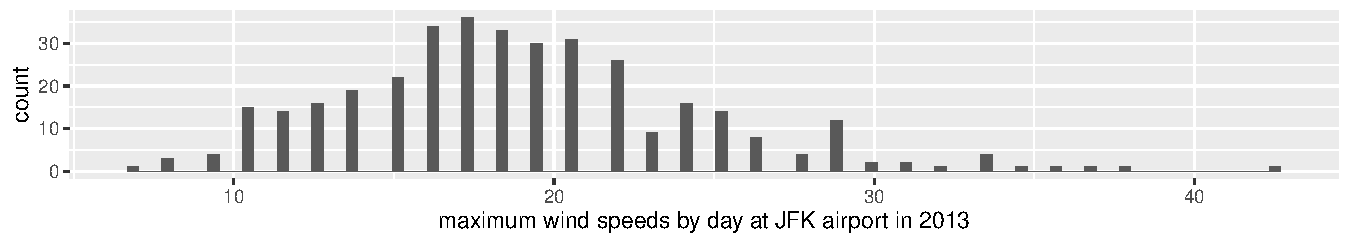
\includegraphics[width = 6in]{windspeeds.pdf}
\end{figure}

\problem\timedsection{10} Above is a histogram of wind speeds at JFK airport measured at midnight for every day in 2013. We fit eight different iid DGPs / models to this data. Below are the models, the maximum likelihood estimates for their parameter(s) and their log likelihood value estimates:

\begin{table}[htp]
\centering
\begin{tabular}{r|cccccccc}
& \multicolumn{8}{c}{Name of Model / DGP}\\
 & Exponential & Normal & Weibull & Gamma & Gumbel & Gompertz & Frechet & Generalized Logistic \\\hline
$\thetahathatmle_1$ & 0.05 & 18.97 & 3.52 & 11.71 & 15.17 & 0.14 & 3.18 & 3.49 \\ 
$\thetahathatmle_2$ &  & 5.59 & 21.01 & 0.62 & 4.84 & 0.05 & 15.59 & 12.22 \\ 
$\thetahathatmle_3$ &  &  &  &  &  &  &  & 4.03 \\ \hline
$\ell(\thetahathatmle_1, \ldots, \thetahathatmle_{K_m}; \xoneton)$ & -1435.12 & -1142.72 & -1148.11 & -1129.28 & -1143.31 & -1200.26 & -1174.37 & -1129.65
\end{tabular}
\end{table}
\FloatBarrier


\vspace{-0.2cm}\benum\truefalsesubquestionwithpoints{9} 

\begin{enumerate}[(a)]
\item All of these models have the same number of parameters $K$.
\item The true model will be one of these eight models candidates.
\item According to the log-likelihood estimates, the best fitting model candidate is the Gamma.
\item According to the AICC metric, the best fitting model candidate is the Generalized Logistic.
\item The asymptotic bias on the true log-likelihood for the normal model is the same as the bias for the Gompertz model.
\item The AIC metric for the generalized logistic model candidate is 2263.30. %false
\item The AIC metric for the exponential model candidate is 2872.24. %true
\item Assuming (b), the probability the exponential model is the true model is negligibly small.
\item AICC values will not significantly differ from the AIC values.
\end{enumerate}
\eenum\instr\pagebreak

%%%%%%%%%%%%%%%%%%%%%%%%


\problem\timedsection{16} In the \qu{Topiramate for the Treatment of Binge Eating Disorder Associated With Obesity: A Placebo-Controlled Study}, the researchers were also interested in adverse effects of the drug Topiramate. One such bad effect is \qu{Upper Respiratory Tract Infection} which we call \emph{infection}. The experimental results are below.

\begin{itemize}
\item In the $n_T = 202$ Topiramate group, there were 75 cases of infection and 
\item in the $n_C = 202$ placebo group that did not take Topiramate, there were 40 cases of infection. 
\end{itemize}
Let $\theta_T$ be the true proportion of infection in Topiramate-takers and $\theta_C$ be the true proportion of infection among non Topiramate-takers.  All numbers below are rounded to the nearest 3 digits.

\vspace{-0.2cm}\benum\truefalsesubquestionwithpoints{13} 

\begin{enumerate}[(a)]
\item When testing $H_a: \theta_T \neq \theta_C$ at $\alpha = 5\%$, a retainment region for $H_0$ is equal to or is approximately $\bracks{-0.086, 0.086}$.%true
\item When testing $H_a: \theta_T \neq \theta_C$ at $\alpha = 5\%$, a retainment region for $H_0$ is equal to or is approximately $\bracks{-0.088, 0.088}$.%true
\item $CI_{\theta_T - \theta_C, 95\%}$ is equal to or is approximately $\bracks{0.087, 0.260}$.%true
\item There is a 95\% chance that the CI estimate in (c) contains the true mean difference $\theta_T - \theta_C$.
\item The estimate of the odds against infection in the Topiramate group is 1.693. %true
\item The estimate of the odds against infection in the Topiramate group is 0.591. %false
\item When testing $H_a: \displaystyle \frac{1 - \theta_T}{\theta_T} \neq \half$ at $\alpha = 5\%$, a retainment region for $H_0$ is equal to or is approximately $\bracks{0.224, 0.776}$.%true
\item The estimate of the risk ratio of infection in the Topiramate group vs the control group is 0.173.%false
\item The estimate of the risk ratio of infection in the Topiramate group vs the control group is 1.875.%true
\item $CI_{\theta_T / \theta_C, 95\%}$ is equal to or is approximately $\bracks{1.255, 2.495}$.%true
\item $CI_{\theta_T / \theta_C, 95\%}$ is equal to or is approximately $\bracks{-0.088, 0.088}$.%false
\item It would be possible to create an exact CI for the risk ratio of infection in the Topiramate group vs the control group given the data here and the concepts learned in class.%false
\item The CI estimator in (j) is more approximate in coverage probability than the CI estimator in (c).
\end{enumerate}
\eenum\instr\pagebreak

%%%%%%%%%%%%%%%%%%%%%%%%

\end{document}

%%%%%%%%%%%%%%%%%%%%%%%%
%%%%%%%%%%%%%%%%%%%%%%%%
%%%%%%%%%%%%%%%%%%%%%%%%
%%%%%%%%%%%%%%%%%%%%%%%%
%%%%%%%%%%%%%%%%%%%%%%%%
%%%%%%%%%%%%%%%%%%%%%%%%
%%%%%%%%%%%%%%%%%%%%%%%%
%%%%%%%%%%%%%%%%%%%%%%%%
%%%%%%%%%%%%%%%%%%%%%%%%
%%%%%%%%%%%%%%%%%%%%%%%%
%%%%%%%%%%%%%%%%%%%%%%%%
%%%%%%%%%%%%%%%%%%%%%%%%
%%%%%%%%%%%%%%%%%%%%%%%%
%%%%%%%%%%%%%%%%%%%%%%%%
%%%%%%%%%%%%%%%%%%%%%%%%
%%%%%%%%%%%%%%%%%%%%%%%%
%%%%%%%%%%%%%%%%%%%%%%%%

